\documentclass{article}
\usepackage{geometry}
\geometry{letterpaper}
\usepackage{graphicx}
\usepackage{amssymb, amsmath}
\usepackage{subfigure}
\usepackage{color}
\usepackage{hyperref}
\usepackage{icml2015}
\usepackage{tikz}

\usetikzlibrary{intersections, backgrounds}

\definecolor{light}{RGB}{199, 153, 199}
\definecolor{dark}{RGB}{180, 31, 180}
\definecolor{gray80}{gray}{0.8}

\graphicspath{{figures/}}

\begin{document}

\icmltitlerunning{The Fragility of Hamiltonian Monte Carlo to Stochastic Data}

\twocolumn[
\icmltitle{The Fragility of Hamiltonian Monte Carlo to Stochastic Data}

\icmlauthor{Michael Betancourt}{betanalpha@gmail.com}
\icmladdress{Department of Statistics, University of Warwick, Coventry, UK CV4 7AL}

\icmlkeywords{Hamiltonian Monte Carlo, Symplectic Integrators, Stochastic Data, ICML}

\vskip 0.3in
]

\begin{abstract}
Abstract
\end{abstract}

Robust to the complexities arising from intricate models, especially those 
common to high dimensional target distributions, Hamiltonian Monte Carlo 
has proven a powerful statistical algorithm.  Still, the computational 
cost of the algorithm can be prohibitive in applications with massive data sets, 
a burden which has motivated the introduction of stochastic data methods.
In this paper I discuss how stochastic data compromises the mathematical 
structure of Hamiltonian Monte Carlo, immediately introducing an uncontrollable
bias that renders the resulting implementations impractical in all but the simplest 
cases.

After first reviewing the mathematical structure of the algorithm and its importance 
towards robust, scalable inference, I introduce two stochastic data
implementations and investigate their overall accuracy relative to the nominal 
implementation that utilizes the full data.  In both cases I demonstrate the fragility 
of the implementation with mathematical arguments and and a simple example.

\section{Hamiltonian Monte Carlo in Theory}

Hamiltonian Monte Carlo \cite{DuaneEtAl:1987, Neal:2011, BetancourtEtAl:2014}
utilizes deterministic, measure-preserving maps to generate efficient 
Markov transitions.  Formally, we begin by complementing a target distribution,
%
\begin{equation*}
\varpi \propto \exp \! \left[ - V ( q ) \right] \mathrm{d}^{n} q,
\end{equation*}
%
with a conditional distribution over auxiliary \textit{momenta} parameters,
%
\begin{equation*}
\varpi_{q} \propto \exp \! \left[ - T (p, q) \right] \mathrm{d}^{n} p.
\end{equation*}
%
Together these define a joint distribution,
%
\begin{align*}
\varpi_{H} 
&\propto \exp \! \left[ - \left( T (q, p) + V (q) \right) \right] \mathrm{d}^{n} q \, \mathrm{d}^{n} p
\\
&\propto \exp \! \left[ - H (q, p) \right] \mathrm{d}^{n} q \, \mathrm{d}^{n} p,
\end{align*}
%
and a \textit{Hamiltonian system} corresponding to the \textit{Hamiltonian},
$ H (q, p) $.  We refer to $T (q, p)$ and $V (q)$ as the \textit{kinetic energy} 
and \textit{potential energy}, respectively.

The Hamiltonian immediately defines a \textit{Hamiltonian flow} on the joint
space,
%
\begin{align*}
\phi^{H}_{t} : (q, p) &\rightarrow (q, p), \forall t \in \mathbb{R}
\\
\phi^{H}_{t} \circ \phi^{H}_{s} &= \phi^{H}_{s + t},
\end{align*}
%
which exactly preserves the joint distribution,
%
\begin{equation*}
\left( \phi^{H}_{t} \right)_{*} \varpi_{H} = \varpi_{H}.
\end{equation*}
%
We can then construct a Markov chain by sampling the auxiliary momenta, 
%
\begin{equation*}
q \rightarrow (q, p), \, p \sim \varpi_{q},
\end{equation*}
%
applying the Hamiltonian flow,
%
\begin{equation*}
(q, p) \rightarrow \phi^{H}_{t} (q, p)
\end{equation*}
%
and then projecting back down to the target space,
%
\begin{equation*}
(q, p) \rightarrow q.
\end{equation*}
%
By construction, the trajectories generated by the Hamiltonian flow 
explore the level sets of the Hamiltonian function, which shadow the
probability mass of the joint distribution.  Because these level sets
can also span large volumes of the joint space, these trajectories
can yield transitions far away from the initial state of the Markov
chain, drastically reducing autocorrelations and producing computationally
efficient Monte Carlo estimators.

When the kinetic energy does not depend on position we say that
the Hamiltonian is \textit{separable}, $H (q, p) = T (p) + V (q)$,  and
the exact Hamiltonian flow can be generated by the \textit{Hamiltonian operator}, 
$\hat{H}$,
%
\begin{equation*}
\phi^{H}_{\tau} = e^{\tau \hat{H}},
\end{equation*}
%
where
%
\begin{align*}
\hat{H} 
&= 
\frac{ \partial H }{ \partial p } \frac{ \partial }{ \partial q}
- \frac{ \partial H }{ \partial q } \frac{ \partial }{ \partial p}
\\
&= 
\frac{ \partial T }{ \partial p } \frac{ \partial }{ \partial q}
- \frac{ \partial V }{ \partial q } \frac{ \partial }{ \partial p}
\\
&\equiv
\quad\, \hat{T} \quad + \quad \hat{V} \quad.
\end{align*}
%
In this paper I consider only separable Hamiltonians, although
the conclusions also carry over to the non-seperable Hamiltonians,
for example those arising in
Riemannian Hamiltonian Monte Carlo \cite{GirolamiEtAl:2011}.

\section{Hamiltonian Monte Carlo in Practice}

The biggest challenge of implementing Hamiltonian Monte Carlo is that the
$e^{\hat{H}}$ is rarely calculable in practice and we must instead resort 
to approximate integration of the Hamiltonian flow.  \textit{Symplectic integrators}, 
which yield numerical trajectories that closely track the true trajectories, are  
of particular importance to any high-performance implementation. 

A particularly transparent strategy for constructing symplectic integrators is to split 
the Hamiltonian into terms with soluble flows which can then be composed together.  
For example, consider the symmetric \textit{Strang} splitting 
\cite{LeimkuhlerEtAl:2004, HairerEtAl:2006},
%
\begin{equation*}
\phi^{V}_{\frac{\epsilon}{2}} \circ 
\phi^{T}_{\epsilon} \circ 
\phi^{V}_{\frac{\epsilon}{2}}
=
e^{\frac{\epsilon}{2} \hat{V} } \circ 
e^{\epsilon \hat{T} } \circ 
e^{\frac{\epsilon}{2} \hat{V} },
\end{equation*}
%
where $\epsilon$ is a small interval of time known as the \textit{step size}.
Appealing to the Baker-Campbell-Hausdorff formula, this symmetric composition yields
%
\begin{align*}
\phi^{V}_{\frac{\epsilon}{2}} \circ 
\phi^{T}_{\epsilon} \circ 
\phi^{V}_{\frac{\epsilon}{2}}
&=
e^{\frac{\epsilon}{2} \hat{V} } \circ 
e^{\epsilon \hat{T} } \circ 
e^{\frac{\epsilon}{2} \hat{V} }
\\
&=
e^{\frac{\epsilon}{2} \hat{V} } \circ 
\exp \left( \epsilon \hat{T} + \frac{\epsilon}{2} \hat{V} 
+ \frac{\epsilon^{2}}{4} \left[ \hat{T}, \hat{V} \right] \right)
+ \mathcal{O} \! \left( \epsilon^{3} \right)
\\
&=
\exp \left( 
\frac{\epsilon}{2} \hat{V} + \epsilon \hat{T} + \frac{\epsilon}{2} \hat{V} 
+ \frac{\epsilon^{2}}{4} \left[ \hat{T}, \hat{V} \right]
+ \frac{1}{2} \left[ \frac{\epsilon}{2} \hat{V}, \epsilon \hat{T} + \frac{\epsilon}{2} \hat{V} 
+ \frac{\epsilon^{2}}{4} \left[ \hat{T}, \hat{V} \right] \right]
\right)
+ \mathcal{O} \! \left( \epsilon^{3} \right)
\\
&=
\exp \left( 
\epsilon \hat{H} 
+ \frac{\epsilon^{2}}{4} \left[ \hat{T}, \hat{V} \right] +\frac{\epsilon^{2}}{4} \left[ \hat{V}, \hat{T} \right] 
+ \frac{\epsilon^{2}}{8} \left[ \hat{V}, \hat{V} \right]
\right)
+ \mathcal{O} \! \left( \epsilon^{3} \right)
\\
&=
e^{ \epsilon \hat{H} }
+ \mathcal{O} \! \left( \epsilon^{3} \right).
\end{align*}
%
Composing this symmetric composition with itself $N = \tau / \epsilon$ times results in 
a symplectic integrator accurate to second-order in the step size for any finite integration 
time, $\tau$,
%
\begin{align*}
\phi^{\widetilde{H}}_{\epsilon, \tau}
&\equiv
\left( \phi^{V}_{\frac{\epsilon}{2}} \circ 
\phi^{T}_{\epsilon} \circ 
\phi^{V}_{\frac{\epsilon}{2}} \right)^{N}
\\
&=
\left( e^{ \epsilon \hat{H} }
+ \mathcal{O} \! \left( \epsilon^{3} \right) \right)^{N}
\\
&=
e^{ \left( N \epsilon \right) \hat{H} }
+ \left( N \epsilon \right) \mathcal{O} \! \left( \epsilon^{2} \right)
\\
&=
e^{ \tau \hat{H} }
+ \tau \mathcal{O} \! \left( \epsilon^{2} \right)
\\
&=
e^{ \tau \hat{H} }
+ \mathcal{O} \! \left( \epsilon^{2} \right).
\end{align*}
%
Remarkably, the resulting numerical trajectories are confined to the level sets
of a \textit{modified Hamiltonian} given by an $\mathcal{O} \! \left( \epsilon^{2} \right)$
perturbation of the exact Hamiltonian \cite{HairerEtAl:2006, BetancourtEtAl:2014b}.

Although such symplectic integrators are accurate they still introduce an
error into the trajectories that can bias the Markov chain and any resulting
Monte Carlo estimators.  In practice this error is typically compensated with
the application of a Metropolis acceptance procedure, accepting the numerical
trajectory only with probability
%
\begin{equation*}
a (p, q) = \min \left(1, 
\exp \! \left( H (q, p) - H \circ \phi^{\widetilde{H}}_{\epsilon, \tau} (q, p) \right) \right).
\end{equation*}

A critical element of this construction is that a large acceptance probability can be 
maintained by simply reducing the step size, $\epsilon$, even as the target distribution 
grows in complexity and dimension \cite{BetancourtEtAl:2014b}.  Because of the
symplectic integrator, Hamiltonian Monte Carlo is robust to the pathologies of complex 
models.  At the same time, the algorithm is fragile to modifications of these
structure-preserving integrators.

\section{Stochastic Hamiltonian Monte Carlo Methods}

A common criticism of Hamiltonian Monte Carlo is that in data-intensive applications 
the potential energy operator,
%
\begin{equation*}
\hat{V} = - \frac{ \partial V }{ \partial q } \frac{ \partial }{ \partial p},
\end{equation*}
%
can become infeasible given the expense of the gradient calculations.  This expense
has fueled a variety of modifications of the algorithm aimed as reducing the cost of 
the potential energy operator, often by any means necessary.

An increasingly popular strategy targets Bayesian applications where the data are 
independently and identically distributed.  In this case the posterior can be manipulated
into a product of contributions from each subset of data, and the potential energy
likewise decomposes into a sum,
%
$V (q) = \sum_{i = 1}^{I} V_{i} (q)$,
%
where each $\left\{ V_{i} \right\}$ depends on only a single subset.  This decomposition 
suggests algorithms which consider not the entirety of the data and the full potential, $V$, 
but rather only a single, randomly chosen subset at a time.

The performance of any such stochastic method depends critically on the details
of the implementation and the structure of the data itself.  Here I consider
the performance of two immediate implementations, one based on subsampling the
data in between Hamiltonian trajectories and one based on subsampling the data
within a single trajectory.  Unfortunately, the performance of both methods leaves
much to be desired.

\subsection{Subsampling Data In Between Trajectories}

Given any subset of the data, we can approximate the potential energy as 
$V \approx I V_{i}$ and then generate trajectories corresponding to the flow of the 
approximate Hamiltonian, $H_{i} = T + I V_{i}$.  In order to avoid parsing the entirely
of the data, the Metropolis acceptance procedure can be neglected and the 
corresponding samples left biased.

Unlike the numerical trajectories from the full Hamiltonian, these stochastic 
trajectories are biased away from the exact trajectories regardless of the
chosen step size.  In particular, the bias of each step,
%
\begin{align*}
e^{\frac{\epsilon}{2} I \hat{V}_{i} } \circ 
e^{\epsilon \hat{T} } \circ 
e^{\frac{\epsilon}{2} I \hat{V}_{i} }
&=
e^{ \epsilon \hat{H}_{i} }
+ \mathcal{O} \! \left( \epsilon^{3} \right)
\\
&=
e^{ \epsilon \hat{H} - \epsilon \widehat{ \Delta V}_{i} }
+ \mathcal{O} \! \left( \epsilon^{3} \right),
\end{align*}
%
where
%
\begin{equation*}
\Delta V_{i} = V - I V_{i},
\end{equation*}
%
persists over an entire trajectory,
%
\begin{equation*}
\left( e^{\frac{\epsilon}{2} I \hat{V}_{i} } \circ 
e^{\epsilon \hat{T} } \circ 
e^{\frac{\epsilon}{2} I \hat{V}_{i} } \right)^{N}
=
e^{ \tau \left( \hat{H} - \widehat{ \Delta V}_{i} \right) }
+ \mathcal{O} \! \left( \epsilon^{2} \right).
\end{equation*}
%
Unless the data are highly redundant and $\Delta V_{i} \approx 0$,
this bias can be large and force vanishing Metropolis acceptance probabilities,
or highly biased expectations if the Metropolis procedure is outright ignored.  
In practice redundancy is guaranteed only when the size of the subsamples
approaches the size of the full data set, but that is exactly the limit when the
computational benefits of subsampling vanishes.

Consider, for example, a simple application where we target a one-dimensional
posterior distribution,
%
\begin{equation} \label{posterior}
p \! \left( \mu | \vec{x} \right) \propto p \! \left( \vec{x} | \mu \right) p\ \! \left( \mu \right),
\end{equation}
%
with the likelihood
%
\begin{equation*}
p \! \left( \vec{x} | \mu \right) = \prod_{n = 1}^{N} \mathcal{N} \! \left( x_{n} | \mu, \sigma^{2} \right)
\end{equation*}
%
and prior
%
\begin{equation*}
p \! \left( \mu \right) = \mathcal{N} \! \left( \mu | m, s^{2} \right). 
\end{equation*}
%
Separating the data into $I = N / B$ batches of size $B$ and decomposing the
prior into $I$ individual terms then gives
%
\begin{equation*}
V_{i} = 
\frac{B}{N} \frac{ \sigma^{2} + N s^{2}  }{ \sigma^{2} s^{2} }
\left( \mu - 
\frac{ \left( \frac{1}{B} \sum_{n = (i - 1) B + 1}^{i B} x_{n} \right) N s^{2}  + m \sigma^{2} }
{ \sigma^{2} + N s^{2} } 
\right)^{2} + \mathrm{const}.
\end{equation*}
%
Here I take $\sigma = 2$, $m = 0$, $s = 1$, and generate $N = 500$ data points
assuming $\mu = 1$.

When the full data are used numerical trajectories generated by the second-order 
symplectic integrator constructed above closely follow the true trajectories 
(Figure \ref{fig:level_sets}a).  Approximating the potential with a subsample of the data 
introduces the aforementioned bias, which shifts the stochastic trajectory away from the 
exact trajectory despite negligible error from the finite step size (Figure \ref{fig:level_sets}b).
Only when the size of each subsample approaches the full data set, and the computational
benefit of subsampling fades, does the stochastic trajectory provide a reasonable
approximation to the exact trajectory (Figure \ref{fig:level_sets}c)

\begin{figure}
\centering
\subfigure[]{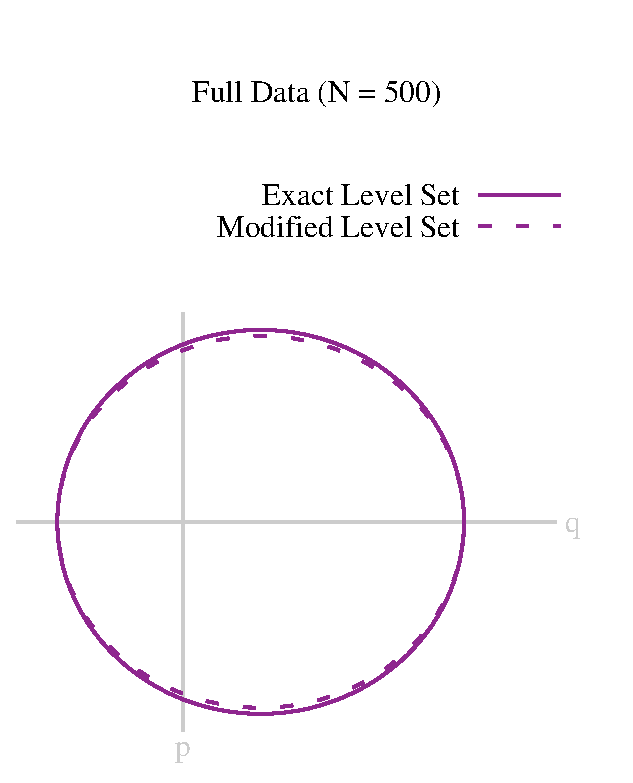
\includegraphics[width=1.75in]{full_level_set.eps}}
\subfigure[]{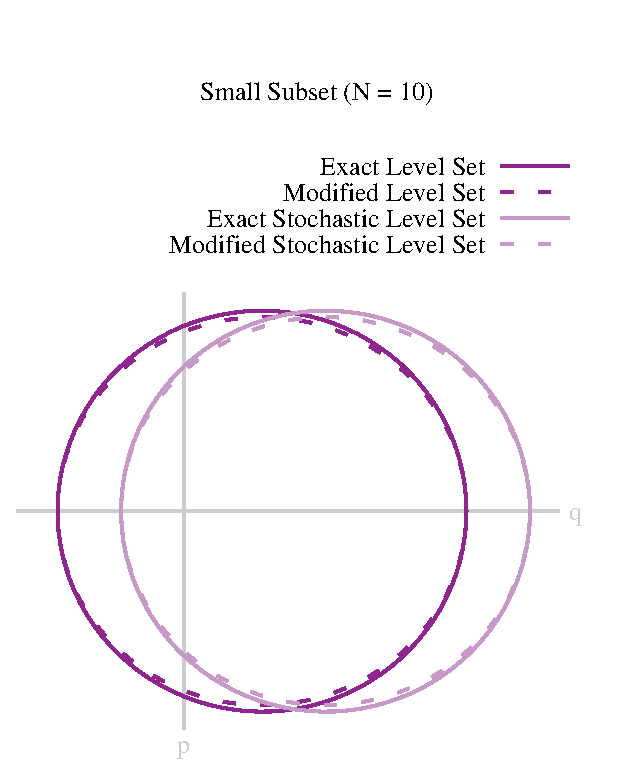
\includegraphics[width=1.75in]{small_batch_level_set.eps}}
\subfigure[]{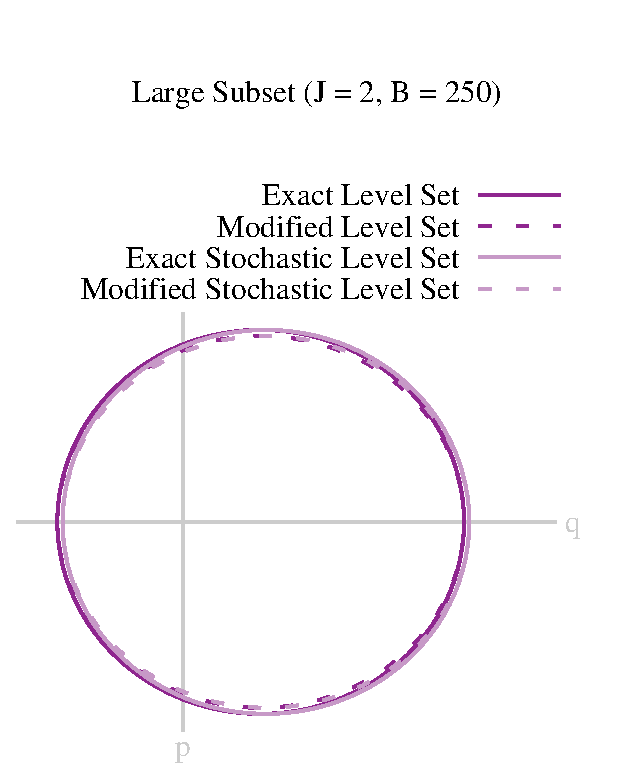
\includegraphics[width=1.75in]{large_batch_level_set.eps}}
\caption{Even in the one-dimensional example, \eqref{posterior}, subsampling
data in between Hamiltonian trajectories introduces significant pathologies.
(a) When the full data are used, numerical Hamiltonian trajectories (dashed line) 
closely track the exact Hamiltonian trajectories (solid line).  Subsampling of the
data introduces a bias in both the exact trajectories and corresponding
numerical trajectories.  (b) If the size of each subsample is small then this bias 
is large, offsetting both the exact and numerical stochastic trajectories. 
(c) Only when the size of the subsamples approaches the size of the full data, 
and any computational benefits from subsampling wane, do the stochastic 
trajectories provide a reasonable emulation of the true trajectories.}
\label{fig:level_sets}
\end{figure}

\subsection{Sampling Potentials within a Single Trajectory}

Given that using a single subsample for an entire trajectory introduces an
irreducible bias, we might next consider subsampling at each step within
a single trajectory in the hope that the bias from each subsample cancels
in expectation.  If the Metropolis acceptance procedure is ignored then this 
approach becomes \textit{stochastic gradient Hamiltonian Monte Carlo}
\cite{ChenEtAl:2014}.

To understand the accuracy of this strategy consider building up such a 
stochastic trajectory one step at a time.  Given the first two randomly-selected 
subsamples, $V_{i}$ and then $V_{j}$, the first two steps of the stochastic
integrator are given by
%
\begin{align*}
\phi^{H_{j}}_{\epsilon} \circ \phi^{H_{i}}_{\epsilon}
&=
e^{ \epsilon \hat{H} - \epsilon  \widehat{ \Delta V}_{j} } 
\circ e^{ \epsilon \hat{H} - \epsilon  \widehat{ \Delta V}_{i} }
+ \mathcal{O} \! \left( \epsilon^{3} \right)
\\
&=
\exp \! \left( 
2 \epsilon \hat{H} - \epsilon \left(  \widehat{ \Delta V}_{i} +  \widehat{ \Delta V}_{j} \right)
+ \frac{\epsilon^{2}}{2} \left[ \hat{H} -  \widehat{ \Delta V}_{j}, \hat{H} - \widehat{ \Delta V}_{i} \right]
\right)
+ \mathcal{O} \! \left( \epsilon^{3} \right)
\\
&=
\exp \! \left( 
2 \epsilon \hat{H} - \epsilon \left( \widehat{ \Delta V}_{i} + \widehat{ \Delta V}_{j} \right)
+ \frac{\epsilon^{2}}{2} \left(
- \left[ \hat{H}, \hat{V}_{\setminus i} \right]
- \left[ \hat{V}_{\setminus j}, \hat{H} \right] \right) \right)
+ \mathcal{O} \! \left( \epsilon^{3} \right),
\end{align*}
%
where we have used the fact that the $\{ \widehat{ \Delta V}_{i} \}$ commute
with each other.  The first three steps are given by
%
\begin{align*}
\phi^{H_{k}}_{\epsilon} \circ \phi^{H_{j}}_{\epsilon} \circ \phi^{H_{i}}_{\epsilon}
&=
\exp \! \left( 
3 \epsilon \hat{H} 
- \epsilon \left( \widehat{ \Delta V}_{i} +  \widehat{ \Delta V}_{j} +  \widehat{ \Delta V}_{k} \right)
+ \frac{\epsilon^{2}}{2} \left(
- \left[ \hat{H}, \widehat{ \Delta V}_{i} \right]
- \left[ \widehat{ \Delta V}_{j}, \hat{H} \right] \right) \right.
\\
& \hspace{13mm} \left.
+ \frac{\epsilon^{2}}{2} \left(
\left[ \hat{H} - \widehat{ \Delta V}_{k}, 2 \hat{H} - \widehat{ \Delta V}_{i} - \widehat{ \Delta V}_{j} \right]
\right)
\right)
+ \mathcal{O} \! \left( \epsilon^{3} \right)
\\
&=
\exp \! \left( 
3 \epsilon \hat{H} 
- \epsilon \left( \widehat{ \Delta V}_{i} + \widehat{ \Delta V}_{j} + \widehat{ \Delta V}_{k} \right)
+ \frac{\epsilon^{2}}{2} \left(
- \left[ \hat{H}, \widehat{ \Delta V}_{i} \right]
- \left[ \widehat{ \Delta V}_{j}, \hat{H} \right] \right) \right.
\\
& \hspace{13mm} \left.
+ \frac{\epsilon^{2}}{2} \left(
- \left[ \hat{H}, \widehat{ \Delta V}_{i} \right]
- \left[ \hat{H}, \widehat{ \Delta V}_{j} \right]
- 2 \left[ \widehat{ \Delta V}_{k}, \hat{H} \right] \right) \right)
+ \mathcal{O} \! \left( \epsilon^{3} \right)
\\
&=
\exp \! \left( 
3 \epsilon \hat{H} 
- \epsilon \left( \widehat{ \Delta V}_{i} + \widehat{ \Delta V}_{j} + \widehat{ \Delta V}_{k} \right)
- \epsilon^{2} \left( \left[ \hat{H}, \widehat{ \Delta V}_{i} \right] 
- \left[ \hat{H}, \widehat{ \Delta V}_{k} \right] \right)
\right) + \mathcal{O} \! \left( \epsilon^{3} \right),
\end{align*}
%
and, letting $i_{n}$ denote the subsample chosen at the $n$-th step, the composition over
an entire trajectory becomes
%
\begin{align*}
\circ_{n = 1}^{N} \phi^{H_{i_{n}}}_{\epsilon}
&=
\exp \! \left( 
\left( N \epsilon \right) \hat{H} 
- \left( N \epsilon \right) \frac{1}{N} \sum_{n = 1}^{N}  \widehat{ \Delta V}_{i_{n}}
+ \left( N \epsilon \right) \epsilon 
\left( \left[ \hat{H}, \widehat{ \Delta V}_{i_{1}} \right] 
- \left[ \hat{H}, \widehat{ \Delta V}_{i_{n}} \right] \right) 
\right)
+ \left(N \epsilon \right) \mathcal{O} \! \left( \epsilon^{2} \right)
\\
&=
\exp \! \left( \tau \hat{H} - \tau \frac{1}{N} \sum_{n = 1}^{N} \widehat{ \Delta V}_{i_{n}}
+ \tau \epsilon 
\left( \left[ \hat{H}, \widehat{ \Delta V}_{i_{1}} \right] 
- \left[ \hat{H}, \widehat{ \Delta V}_{i_{N}} \right] \right)
\right)
+ \mathcal{O} \! \left( \epsilon^{2} \right)
\\
&=
\exp \! \left( \tau \hat{H} + \tau B_{1} + \tau B_{2} \right)
+ \mathcal{O} \! \left( \epsilon^{2} \right),
\end{align*}
%
where
%
\begin{equation*}
B_{1} = - \sum_{n = 1}^{N} \widehat{ \Delta V}_{i_{n}}
\end{equation*}
%
and
%
\begin{equation*}
B_{2} = \epsilon 
\left( \left[ \hat{H}, \widehat{ \Delta V}_{i_{1}} \right] 
- \left[ \hat{H}, \widehat{ \Delta V}_{i_{N}} \right] \right).
\end{equation*}
%
As in the previous case, the stochastic approximation of the potential energy
introduces bias into the numerical trajectories, although the bias here is 
fundamentally different.

Although the second source of bias, $B_{2}$, is immediately rectified by appending the 
stochastic trajectory with an update from the initial subsample such that $i_{N} = i_{1}$, 
the first source of bias, $B_{1}$, is not so easily remedied.  Noting that
%
\begin{align*}
\frac{1}{N} \sum_{n = 1}^{N}  \widehat{ \Delta V}_{i_{n}}
&=
\frac{1}{N} \sum_{n = 1}^{N} \left( \hat{V} - I \hat{V}_{i_{n}} \right)
\\
&=
\hat{V} - \frac{I}{N} \sum_{n = 1}^{N} \hat{V}_{i_{n}}
\\
&=
- \left( \frac{ \partial V }{ \partial q }  - \frac{I}{N} \sum_{n = 1}^{N} \frac{ \partial V_{i} }{ \partial q }
\right) \frac{ \partial }{ \partial p },
\end{align*}
%
we see that $B_{1}$ vanishes only when the average gradient of the selected 
subsamples yields the gradient of the full potential (Figure \ref{fig:subsampled_gradients}).

\begin{figure*}
\centering
%
\subfigure[]{
%\begin{tikzpicture}[scale=0.20, thick, show background rectangle]
\begin{tikzpicture}[scale=0.22, thick]
  
  \draw [light, thick] plot [smooth, tension=1.1] coordinates {(0,5) (10, 10) (21, 8) (25, 8)}
  node[right] { Stochastic };

  \draw [dark, thick] plot [smooth, tension=1.1] coordinates {(0,0) (10, 7) (20, 5) (24, 5)}
  node[right] { Exact };
  
  \draw[->, color=gray80, thick] (10, 10) -- +(3, 3);
  \draw[->, color=gray80, thick] (10, 10) -- +(3, -3);
  \draw[->, color=gray80, thick] (10, 10) -- +(1, 4);
  \draw[->, color=gray80, thick] (10, 10) -- +(-1, 5);
  \draw[->, color=gray80, thick] (10, 10) -- +(1, -2);
  \draw[->, color=gray80, thick] (10, 10) -- +(-1, -2);
  
  \draw[->, color=black, thick] (10, 10) -- +(3, 0.5);
  
\end{tikzpicture}
}
\subfigure[]{
%\begin{tikzpicture}[scale=0.20, thick, show background rectangle]
\begin{tikzpicture}[scale=0.22, thick]

  \draw [light, thick] plot [smooth, tension=0.8] coordinates {(0,5) (2, 6.75) (4, 8) (6, 8.95) 
  (8, 9.6) (10, 10) (12, 10.7) (14, 13) (16, 17)}
  node[right] { Stochastic };

  \draw [dark, thick] plot [smooth, tension=1.1] coordinates {(0,0) (10, 7) (20, 5) (24, 5)}
  node[right] { Exact };
  
  \draw[->, color=gray80, thick] (10, 10) -- +(1, 4);
  \draw[->, color=gray80, thick] (10, 10) -- +(-1, 5);
  \draw[->, color=gray80, thick] (10, 10) -- +(1, -2);
  
  \draw[->, color=black, thick] (10, 10) -- +(2, 2);
  
\end{tikzpicture}
}
\caption{The bias induced by subsampling data within a single Hamiltonian
trajectory depends on how precisely the gradients of the subsampled potential
energies integrate to the gradient of the true potential energy.
(a) When the stochastic gradients integrate to the true gradient, the
stochastic trajectory will follow the true trajectory and the bias will be small. 
(b) Conversely, if the stochastic gradients do not integrate to the true
potential energy then the stochastic trajectory will drift away from the true
trajectory and induce a large bias.  As the dimensionality of the target distribution
grows, maintaining a small bias becomes increasingly more difficult unless
every subsample is used within a stochastic trajectory.}
\label{fig:subsampled_gradients}
\end{figure*}

One way of ensuring this condition is to use each subsample the same number
of times within a single trajectory.  In particular, both biases identically vanish if 
we use each subsample twice in a symmetric composition of the form
%
\begin{equation*}
\left( \circ_{n = 1}^{N} \phi^{H_{n}}_{\epsilon} \right)
\circ 
\left( \circ_{n = 1}^{N} \phi^{H_{N + 1 - n}}_{\epsilon} \right).
\end{equation*}
%
Because this composition requires using all of the subsamples it does not provide
any computational savings and seems rather at odd with the original stochastic 
motivation of the algorithm. 

Indeed, this symmetric composition is not stochastic at all and actually corresponds 
to a rather elaborate symplectic integrator with an effective step size of $I \epsilon$, 
where the potential energy from each subsample generates its own flow.  Removing 
intermediate steps from this symmetric, stochastic trajectory 
(Figure \ref{fig:symmetric_stochastic}a) reveals the level set of the corresponding
modified Hamiltonian (Figure \ref{fig:symmetric_stochastic}b).  Because this
symmetric composition integrates the full Hamiltonian system, the error is 
once again controllable and vanishes as the step size is decreased
(Figure \ref{fig:symmetric_stochastic}c).

\begin{figure}
\centering
\subfigure[]{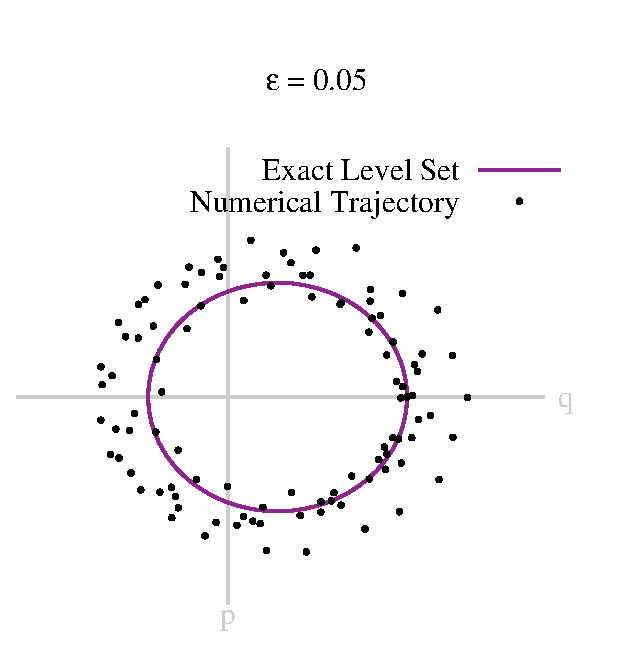
\includegraphics[width=1.95in]{symmetric_trajectory.eps}}
\subfigure[]{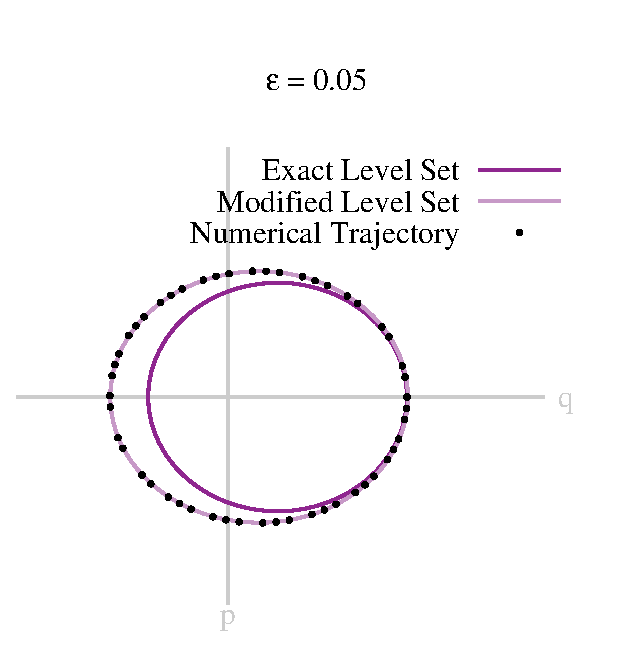
\includegraphics[width=1.95in]{symmetric_level_set.eps}}
\subfigure[]{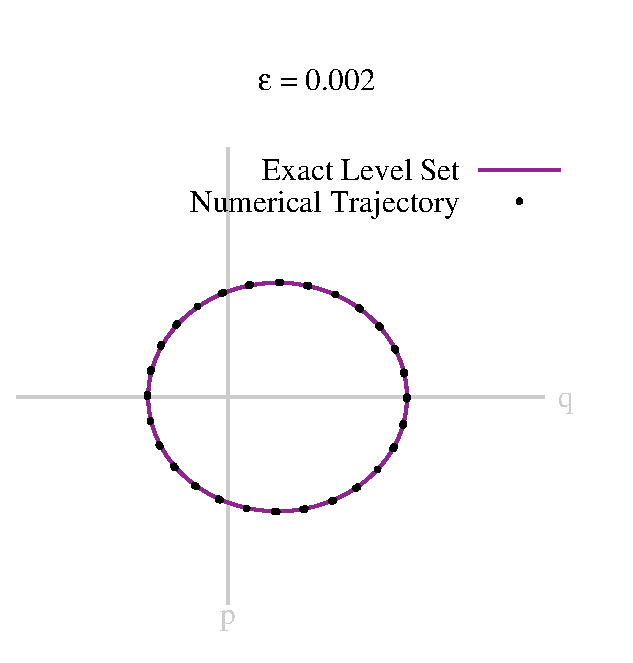
\includegraphics[width=1.95in]{symmetric_level_set_scaled.eps}}
\caption{The symmetric composition of flows from each subsample eliminates
all bias in the stochastic trajectory because it implicitly reconstructs a symplectic
integrator.  Refining all (a) steps in a stochastic trajectory (b) to
only those occurring after a symmetric sweep of the subsamples reveals
the level set of the modified Hamiltonian corresponding to the implicit
symplectic integrator.  Because of the vanishing bias, (c) the error in the
stochastic trajectory vanishes as the step size decreases towards zero. }
\label{fig:symmetric_stochastic}
\end{figure}

If we want to a computational benefit from subsampling then we need to
utilize only a small number of subsamples without the bias growing too
large.  Because the bias cannot be controlled by the tuning the step size
(Figure \ref{fig:subsample_trajectory}), the rescaling used in stochastic
Langevin Monte Carlo methods 
\cite{WellingEtAl:2011, TehEtAl:2014, VollmerEtAl:2015} is not applicable; 
instead our only hope lies in the redundancy of the data itself.  

When the data are highly redundant the gradient of the potential energy from 
a few subsamples may reasonably emulate the gradient of the potential energy 
from the full data.  This limits the potential applicability of this stochastic approach 
to the asymptotic regime where the data expands relative to the model complexity, 
sometimes known as the \textit{tall data} regime.

\begin{figure}
\centering
\subfigure[]{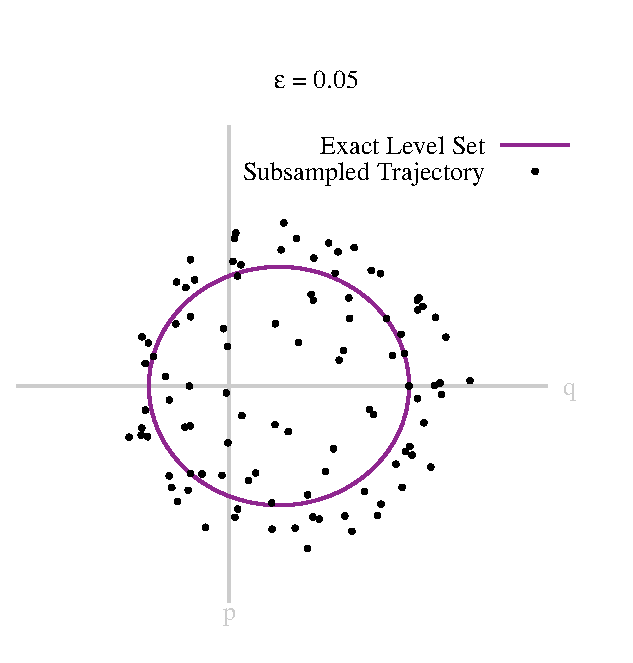
\includegraphics[width=2.9in]{subsample_trajectory.eps}}
\subfigure[]{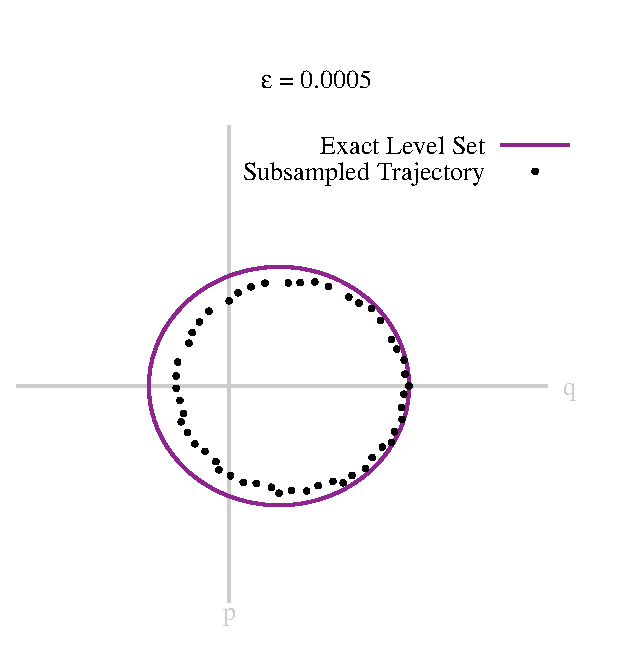
\includegraphics[width=2.9in]{subsample_trajectory_step3.eps}}
\caption{(a) Utilizing only a few subsamples yields numerical trajectories
biased away from the exact trajectories.  (b) Unlike the error introduced by
a full symplectic integrator, this bias is irreducible and cannot be controlled
by tuning the step size.  The performance of such an algorithm is limited by 
the size of the bias which itself depends on the redundancy of the data.}
\label{fig:subsample_trajectory}
\end{figure}

\section{Conclusion}

Symplectic integrators admit a structure-preserving implementation of
Hamiltonian Monte Carlo that is amazingly robust to model complexity,
especially in many dimensions and with sparse data.  When the
underlying symplectic integrator is compromised, however, the algorithm
can quickly fail, making it fragile to various modifications, including those
relying on stochastic data.

The one regime where stochastic variants of Hamiltonian Monte Carlo
may hold promise is the tall data regime, where the data are highly
redundant and stochastic subsampling does not appreciably lessen
the available information.  This is 

Consistent with a growing volume of Markov Chain Monte Carlo literature 
\cite{NeiswangerEtAl:2013, BardenetEtAl:2014}, these stochastic
subsampling methods have potential applicability only in the tall data regime 
where the data are highly redundant.  Even then, care must be taken to 
validate that the bias induced by subsampling the data is understood,
a validation sensitive to not just the target distribution but also each
expectation desired by the application at hand.

Unfortunately many of the problems at the frontiers of applied statistics are 
in the \textit{wide data} regime where data are sparse relative to model 
complexity.  Here subsampling methods are impractical and only an
implementation of Hamiltonian Monte Carlo using the full data offers
precise estimation of posterior expectations.  If such an implementation
is too expensive then we must step back and, with data preprocessing
in mind, ask different statistical questions whose answers are computationally 
feasible.

%\section*{Acknowledgements}

%I thank Matt Johnson and Sam Livingstone for careful readings of this
%manuscript and helpful comments.  
%I am supported under EPSRC grant EP/J016934/1

\bibliography{stochastic_integrators}
\bibliographystyle{icml2015}

%%%%%%%%%%%%%%%%%%%%%%%%%%%%%%%%%%%%%%%%
%%%%%%%%%%%%%%%%%%%%%%%%%%%%%%%%%%%%%%%%
%%   Calculation assuming that [V_{\i}, V_{\j} ] \neq 0
%%%%%%%%%%%%%%%%%%%%%%%%%%%%%%%%%%%%%%%%
%%%%%%%%%%%%%%%%%%%%%%%%%%%%%%%%%%%%%%%%

\begin{comment}

\begin{align*}
\phi^{H_{j}}_{\epsilon} \circ \phi^{H_{i}}_{\epsilon}
&=
e^{ \epsilon \hat{H} - \epsilon \hat{V}_{\setminus j} } 
\circ e^{ \epsilon \hat{H} - \epsilon \hat{V}_{\setminus i} }
+ \mathcal{O} \! \left( \epsilon^{3} \right)
\\
&=
\exp \! \left( 
2 \epsilon \hat{H} - \epsilon \left( \hat{V}_{\setminus i} + \hat{V}_{\setminus j} \right)
+ \frac{\epsilon^{2}}{2} \left[ \hat{H} -\hat{V}_{\setminus j}, \hat{H} -\hat{V}_{\setminus i} \right]
\right)
+ \mathcal{O} \! \left( \epsilon^{3} \right)
\\
&=
\exp \! \left( 
2 \epsilon \hat{H} - \epsilon \left( \hat{V}_{\setminus i} + \hat{V}_{\setminus j} \right)
+ \frac{\epsilon^{2}}{2} \left(
- \left[ \hat{H}, \hat{V}_{\setminus i} \right]
- \left[ \hat{V}_{\setminus j}, \hat{H} \right]
+ \left[ \hat{V}_{\setminus j}, \hat{V}_{\setminus i} \right] \right)
\right)
+ \mathcal{O} \! \left( \epsilon^{3} \right)
\end{align*}
%
and
\begin{align*}
\phi^{H_{k}}_{\epsilon} \circ \phi^{H_{j}}_{\epsilon} \circ \phi^{H_{i}}_{\epsilon}
&=
\exp \! \left( 
3 \epsilon \hat{H} 
- \epsilon \left( \hat{V}_{\setminus i} + \hat{V}_{\setminus j} + \hat{V}_{\setminus k} \right)
+ \frac{\epsilon^{2}}{2} \left(
- \left[ \hat{H}, \hat{V}_{\setminus i} \right]
- \left[ \hat{V}_{\setminus j}, \hat{H} \right]
+ \left[ \hat{V}_{\setminus j}, \hat{V}_{\setminus i} \right] \right) \right.
\\
& \hspace{13mm} \left.
+ \frac{\epsilon^{2}}{2} \left(
\left[ \hat{H} - \hat{V}_{\setminus k}, 2 \hat{H} - \hat{V}_{\setminus i} - \hat{V}_{\setminus j} \right]
\right)
\right)
+ \mathcal{O} \! \left( \epsilon^{3} \right)
\\
&=
\exp \! \left( 
3 \epsilon \hat{H} 
- \epsilon \left( \hat{V}_{\setminus i} + \hat{V}_{\setminus j} + \hat{V}_{\setminus k} \right)
+ \frac{\epsilon^{2}}{2} \left(
- \left[ \hat{H}, \hat{V}_{\setminus i} \right]
- \left[ \hat{V}_{\setminus j}, \hat{H} \right]
+ \left[ \hat{V}_{\setminus j}, \hat{V}_{\setminus i} \right] \right) \right.
\\
& \hspace{13mm} \left.
+ \frac{\epsilon^{2}}{2} \left(
- \left[ \hat{H}, \hat{V}_{\setminus i} \right]
- \left[ \hat{H}, \hat{V}_{\setminus j} \right]
- 2 \left[ \hat{V}_{\setminus k}, \hat{H} \right]
+ \left[ \hat{V}_{\setminus k}, \hat{V}_{\setminus i} \right]
+ \left[ \hat{V}_{\setminus k}, \hat{V}_{\setminus j} \right]
\right)
\right)
+ \mathcal{O} \! \left( \epsilon^{3} \right)
\\
&=
\exp \! \left( 
3 \epsilon \hat{H} 
- \epsilon \left( \hat{V}_{\setminus i} + \hat{V}_{\setminus j} + \hat{V}_{\setminus k} \right)
- \epsilon^{2} \left( \left[ \hat{H}, \hat{V}_{\setminus i} \right] - \left[ \hat{H}, \hat{V}_{\setminus k} \right] \right)
\right.
\\
& \hspace{13mm} \left.
+ \frac{\epsilon^{2}}{2} \left(
+ \left[ \hat{V}_{\setminus j}, \hat{V}_{\setminus i} \right] 
+ \left[ \hat{V}_{\setminus k}, \hat{V}_{\setminus i} \right]
+ \left[ \hat{V}_{\setminus k}, \hat{V}_{\setminus j} \right]
\right)
\right)
+ \mathcal{O} \! \left( \epsilon^{3} \right),
\end{align*}
%
or, in general,
%
\begin{align*}
\circ_{n = 1}^{N} \phi^{H_{I_{n}}}_{\epsilon}
&=
\exp \! \left( \left( N \epsilon \right) \hat{H} - \left( N \epsilon \right) \frac{1}{N} \sum_{n = 1}^{N} V_{\setminus I_{n}}
+ \left( N \epsilon \right) \epsilon 
\left( \left[ \hat{H}, \hat{V}_{\setminus I_{1}} \right] - \left[ \hat{H}, \hat{V}_{\setminus I_{n}} \right] \right)
\right.
\\
& \hspace{13mm} \left.
+ \left( N \epsilon \right) \frac{\epsilon}{2} \frac{1}{N} \sum_{n=1}^{N} \sum_{m=1}^{n}
\left[ \hat{V}_{\setminus I_{n}}, \hat{V}_{\setminus I_{m}} \right] \right)
+ \left(N \epsilon \right) \mathcal{O} \! \left( \epsilon^{2} \right)
\\
&=
\exp \! \left( \tau \hat{H} - \tau \frac{1}{N} \sum_{n = 1}^{N} V_{\setminus I_{n}}
+ \tau \epsilon 
\left( \left[ \hat{H}, \hat{V}_{\setminus I_{1}} \right] - \left[ \hat{H}, \hat{V}_{\setminus I_{n}} \right] \right)
\right.
\\
& \hspace{13mm} \left.
+ \tau \frac{\epsilon}{2} \frac{1}{N} \sum_{n=1}^{N} \sum_{m=1}^{n}
\left[ \hat{V}_{\setminus I_{n}}, \hat{V}_{\setminus I_{m}} \right] \right)
+ \mathcal{O} \! \left( \epsilon^{2} \right).
\end{align*}

In contrast to the deterministic integrator, the stochastic integrator has errors at both
zeroth and first-orders with the potential to drastically reduce the ultimate accuracy.
Let's first consider the zeroth-order error, which can be manipulated into
%
\begin{align*}
\frac{1}{N} \sum_{n = 1}^{N}  \widehat{ \Delta V}_{i}
&=
\frac{1}{N} \sum_{n = 1}^{N} \left( V - V_{I_{n}} \right)
\\
&=
V - \frac{1}{N} \sum_{n = 1}^{N} V_{I_{n}}.
\end{align*}
%
In words, the zeroth-order error vanishes only when the selected subsets yield an
unbiased estimator of the true potential energy.  In practice this requires that either
the data are heavily redundant, in which case a few subsamples may be used, or
all subsamples are used exactly once.

This leaves the first-order error, which is itself comprised of two terms.  The first
term vanishes if we append the trajectory with an update from the first subsample
used, which is an simple and cheap modification to the algorithm.  Unfortunately
the second term remains and vanishes only when each subsample is identical,
which is again the limit of fully redundant data.  \textbf{Can this be manipulated
into a variance-like term?}

\end{comment}

\end{document}
